%%%% Paramétrage du TD %%%%
\def\xxactivite{TD 11 \ifprof -- Corrigé \else \fi} % \normalsize \vspace{-.4cm}
\def\xxauteur{\textsl{Xavier Pessoles}}


\def\xxnumchapitre{Chapitre 1 \vspace{.2cm}}
\def\xxchapitre{\hspace{.12cm} Correction des systèmes}

\def\xxcompetences{%
\textsl{%
\textbf{Savoirs et compétences :}\\ \vspace{-.4cm}
\begin{itemize}[label=\ding{112},font=\color{ocre}]
\item \textit{C1-02 : }Proposer une démarche de réglage d'un correcteur.
\item \textit{C2-04 : }Mettre en œuvre une démarche de réglage d’un correcteur.
\end{itemize}
}}

\def\xxtitreexo{Téléchirurgie robotisée au contact d’organes mobiles}
\def\xxsourceexo{\hspace{.2cm} CCP -- PSI 2015}
\def\xxauteur{\textsl{Xavier Pessoles}}

\def\xxfigures{
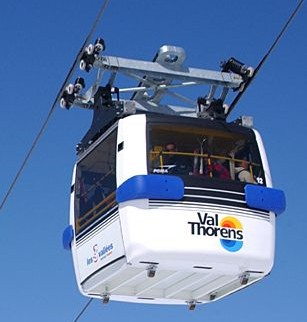
\includegraphics[width=.35\linewidth]{fig_00}
}%figues de la page de garde


\input{\repRel/Style/pagegarde_TD}
\setcounter{numques}{0}


\setlength{\columnseprule}{.1pt}

\pagestyle{fancy}
\thispagestyle{plain}

\vspace{4.9cm}

\def\columnseprulecolor{\color{ocre}}
\setlength{\columnseprule}{0.4pt} 

%%%%%%%%%%%%%%%%%%%%%%%

\setcounter{exo}{0}
\begin{multicols}{2}

%\section*{}

\subsection*{Présentation}


\subsection*{Réalisation de la commande de l’esclave}
\begin{obj}
Concevoir la commande du dispositif esclave de façon à satisfaire l’ensemble des
exigences incluses dans l’exigence « Commande » (id 1.1).
\end{obj}

\begin{center}
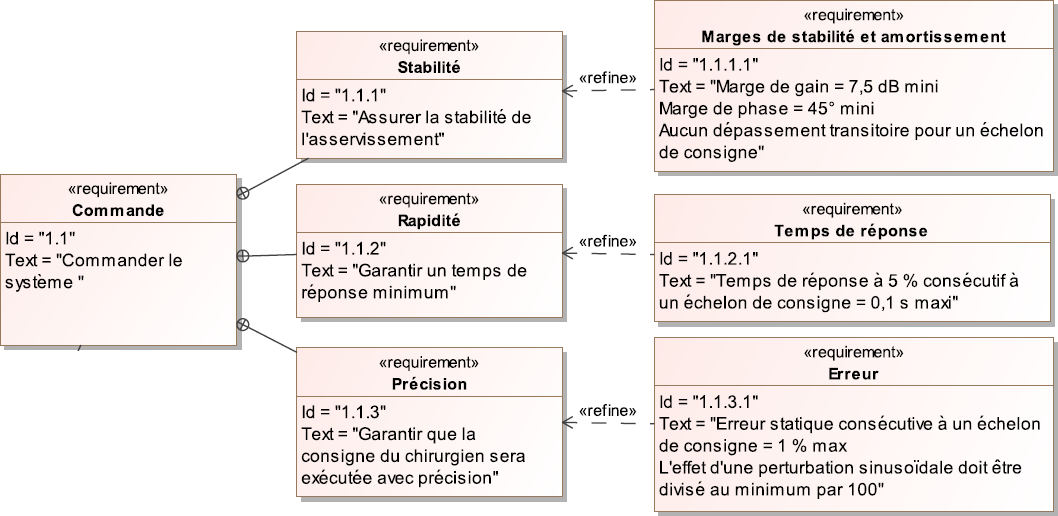
\includegraphics[width=1.0\linewidth]{req_01}
\end{center}

\begin{center}
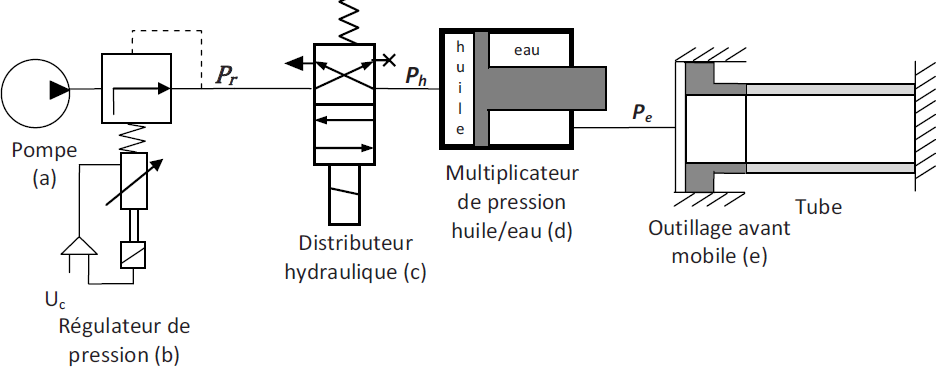
\includegraphics[width=1.0\linewidth]{fig_01}
\end{center}


\subsection*{Modélisation et étude des performances du système sans correction}
\begin{obj}
Identifier les performances non satisfaites afin de choisir un correcteur adapté.
\end{obj}

La modélisation permettant de relier la consigne $x_m(t)$ issue du dispositif maître au déplacement
$x_v(t)$ de l’organe terminal est représentée par le schéma-blocs suivant.

\begin{center}
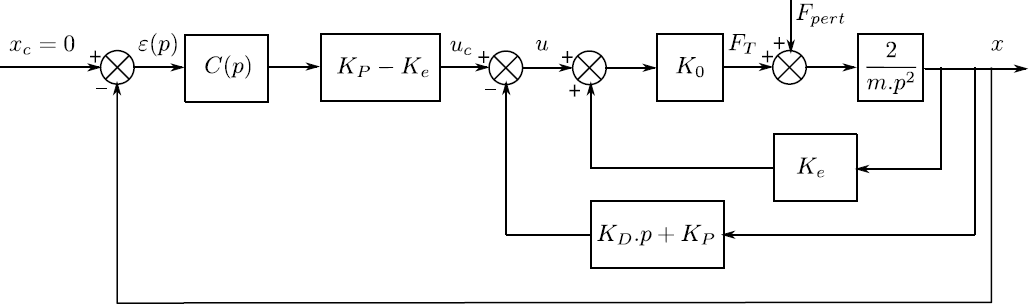
\includegraphics[width=1.0\linewidth]{fig_02}
\end{center}

\begin{itemize}
\item $H_{\text{ad}}(p) = k_a = \SI{1}{Nm^{-1}}$ permet d’adapter la consigne position en consigne force ;
\item $H_S(p) = \dfrac{X_S(p)}{F_S(p)}=\dfrac{k_S}{p\left( m_S +b_S\right)}$ avec $k_S = \SI{1}{m.N^{-1}}$, $m_S = \SI{0,152}{kg}$ et $b_S = \SI{1,426}{Nsm^{-1}}$;
\item $k_e = \SI{200}{N.m^{-1}}$.
\end{itemize}


\question{Simplifier le schéma-blocs précédant pour lui donner la forme illustrée par la figure suivante.
Exprimer $H_t(p)$ et $H(p)$ en fonction de $k_e$, $k_a$ et $H_S(p)$.}
\ifprof
\begin{corrige}
\end{corrige}
\else
\fi


\begin{center}
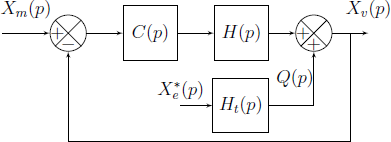
\includegraphics[width=.8\linewidth]{fig_03}
\end{center}

Pour la suite du problème, on prendra : $H(p) = \dfrac{1}{m_S p^2 + b_S p + k_e}$.

\subsection*{Vérification des exigences sans correction : $C(p) =~1$}

\question{Déterminer la fonction de transfert en boucle fermée (avec une perturbation nulle :
$X^{*}_e(p)=0$) : $F_{\text{BF1}}(p) =\dfrac{X_v(p)}{X_m(p)}$, puis la mettre sous forme canonique de façon à identifier les paramètres caractéristiques : gain statique ($K$), pulsation propre ($\omega_0$) et coefficient d’amortissement
($z$). Faire l’application numérique.}
\ifprof
\begin{corrige}
\end{corrige}
\else
\fi

\question{En vous aidant des abaques de la figure suivante, vérifier les exigences « stabilité »
(uniquement l’amortissement), « rapidité » et « précision » (uniquement l’erreur statique).}
\ifprof
\begin{corrige}
\end{corrige}
\else
\fi


\begin{center}
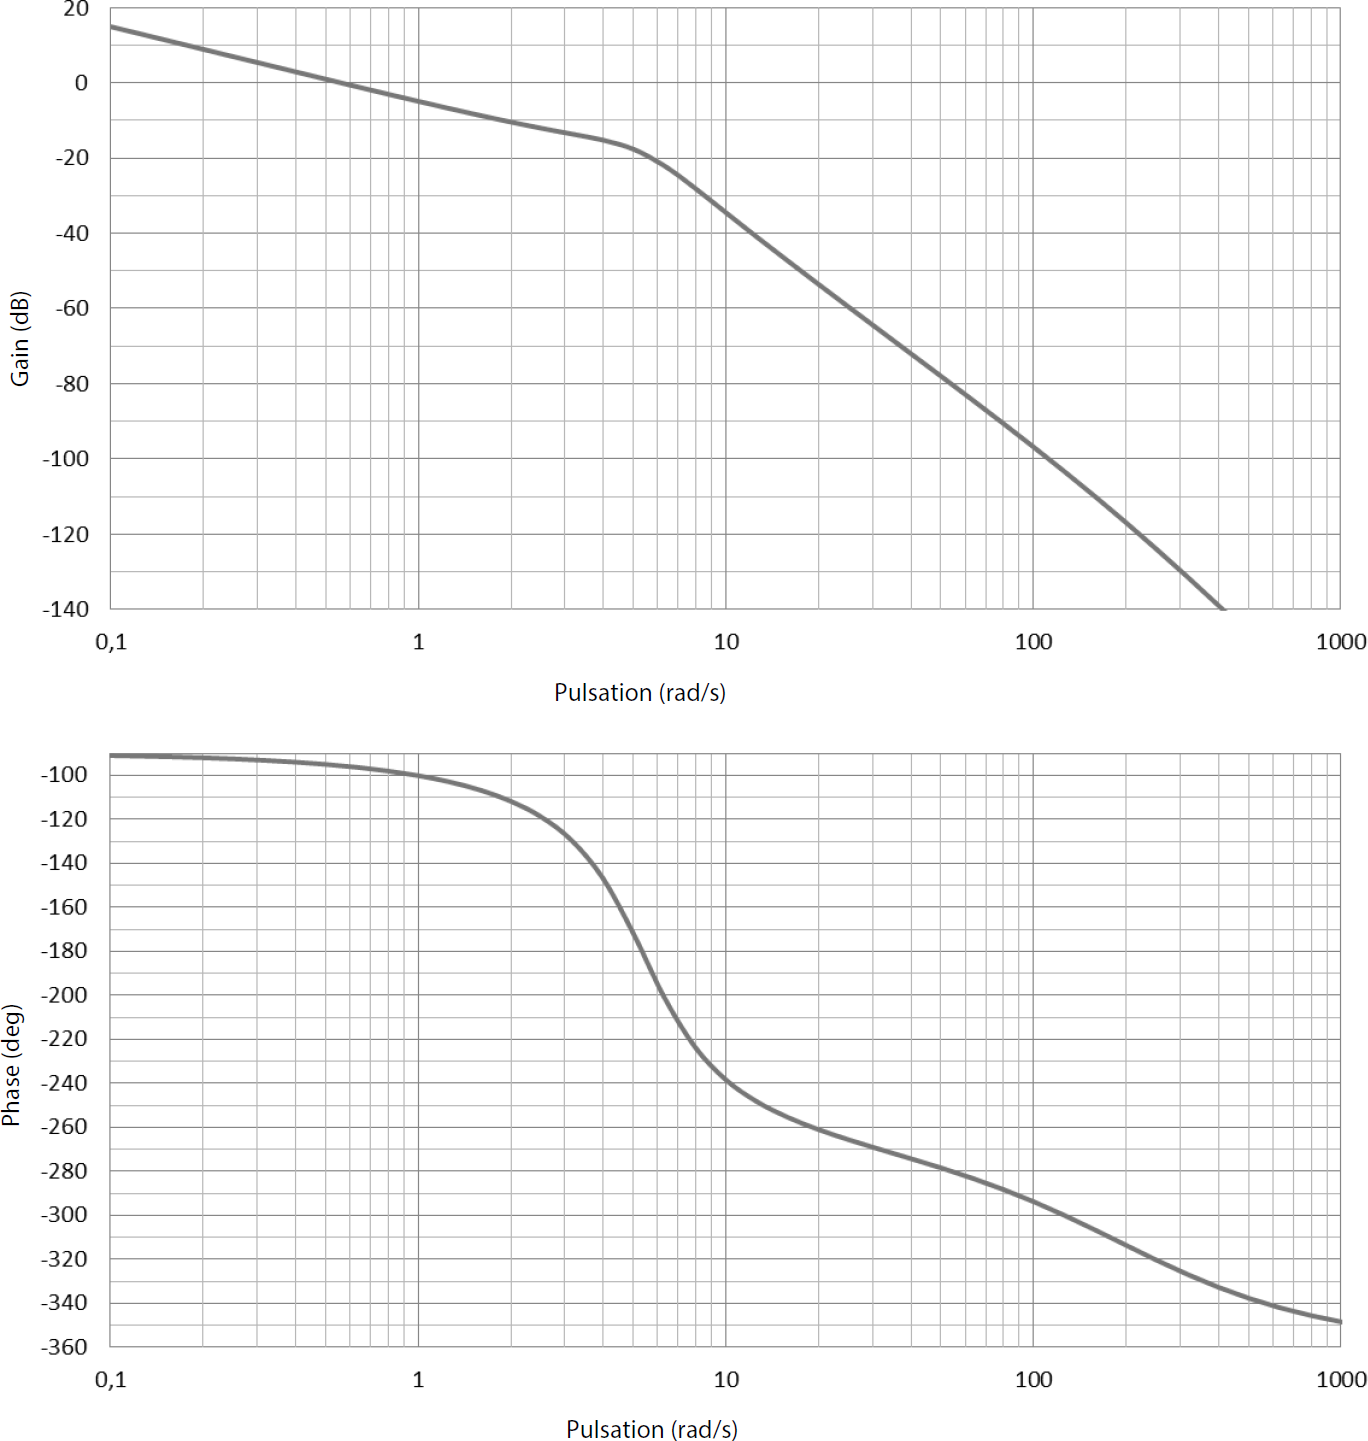
\includegraphics[width=1.0\linewidth]{fig_04}
\end{center}


\begin{center}
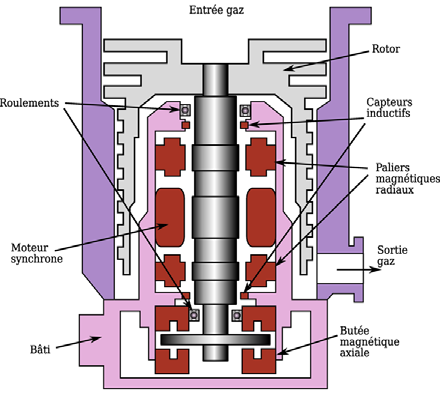
\includegraphics[width=1.0\linewidth]{fig_05}
\end{center}

\subsection*{Modélisation et étude des performances du système avec correction intégrale : $C(p) = \dfrac{K_i}{p}$}

\begin{obj}
Vérifier la capacité d’une correction intégrale à atteindre les exigences.
\end{obj}

\question{Les résultats d’une simulation pour un gain $K_i = 100$ sont donnés sur les figures suivantes. Vérifier les exigences «~stabilité~», «~rapidité~», «~précision~» (uniquement l’erreur statique).}
\ifprof
\begin{corrige}
\end{corrige}
\else
\fi

\question{Justifier exhaustivement le tracé des diagrammes de Bode. Tracer le diagramme asymptotique.}
\ifprof
\begin{corrige}
\end{corrige}
\else
\fi

\begin{center}
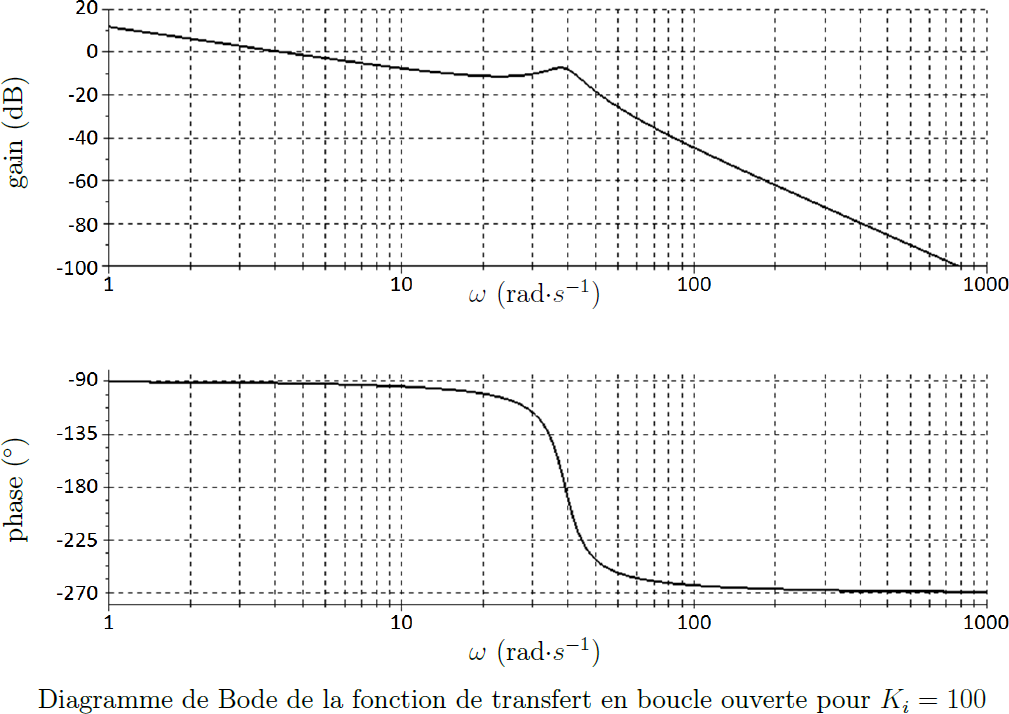
\includegraphics[width=1.0\linewidth]{dr_01}
\end{center}

\begin{center}
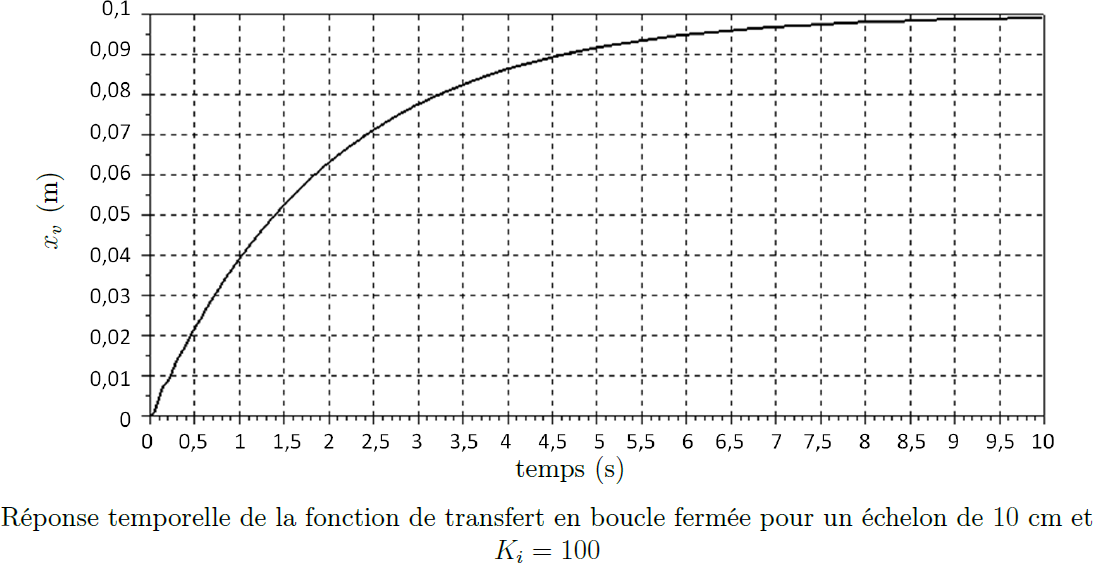
\includegraphics[width=1.0\linewidth]{dr_02}
\end{center}


\question{Pour améliorer la rapidité, il faut augmenter le gain $K_i$. Déterminer la valeur $K_{\text{imax}}$ du
coefficient $K_i$ qui permet de respecter les marges de stabilité.}
\ifprof
\begin{corrige}
\end{corrige}
\else
\fi

\question{En analysant la courbe suivante, conclure sur la capacité du correcteur à valider simultanément les exigences de «~stabilité~» et de «~rapidité~».}
\ifprof
\begin{corrige}
\end{corrige}
\else
\fi
\begin{center}
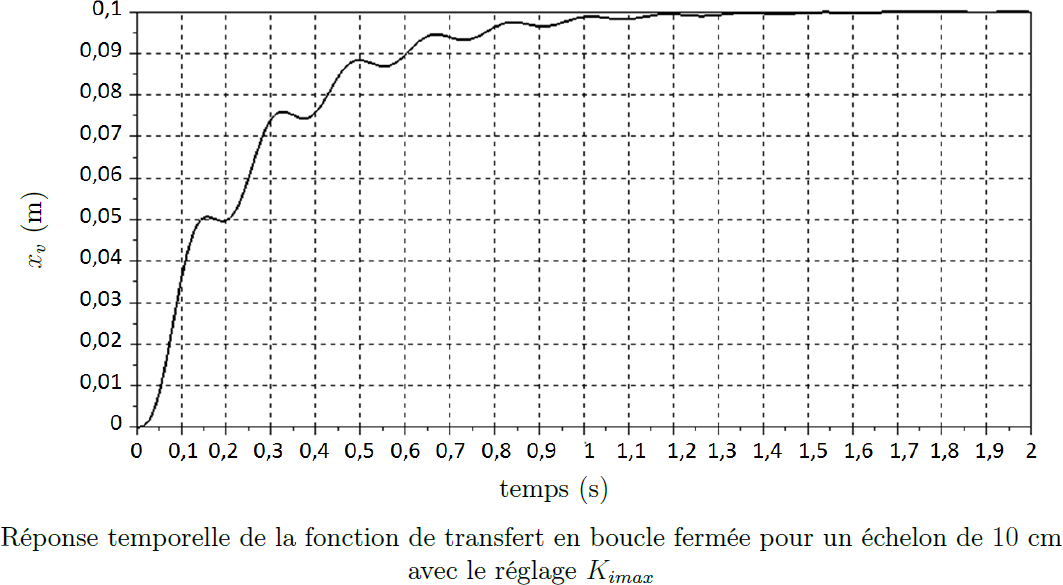
\includegraphics[width=1.0\linewidth]{dr_03}
\end{center}


\question{Le diagramme de Bode de la figure suivante représente la réponse fréquentielle (courbe de gain
uniquement) de la fonction $F_{\text{BF2}} (j\omega) = \dfrac{X_v(j\omega)}{X_e^*(j\omega)}$
pour $K_i = K_{\text{imax}}$. Quelle sera l’atténuation minimale $\left|F_{\text{BF2}}\left(j\omega\right)\right|_{\text{min}}$
de la perturbation $x_e^*$ (en \%) sur l’intervalle $[\SI{1,25}{rad.s^{-1}};\SI{12,5}{rad.s^{-1}}]$.
Conclure sur la validation de l’exigence de « précision ».}
\ifprof
\begin{corrige}
En \SI{1,25}{rad.s^{-1}} l'atténuation est de $\SI{-55}{dB}$. On a $20\log K = -55$ soit $K=0,002$ (inférieur à 1\%). 
En \SI{12,5}{rad.s^{-1}} l'atténuation est de $\SI{-30}{dB}$. On a $20\log K = -30$ soit $K=0,03$ (supérieur à 1\%). 

Le critère d'atténuation n'est pas vérifié sur l'ensemble de l'intervalle.
\end{corrige}
\else
\fi



\begin{center}
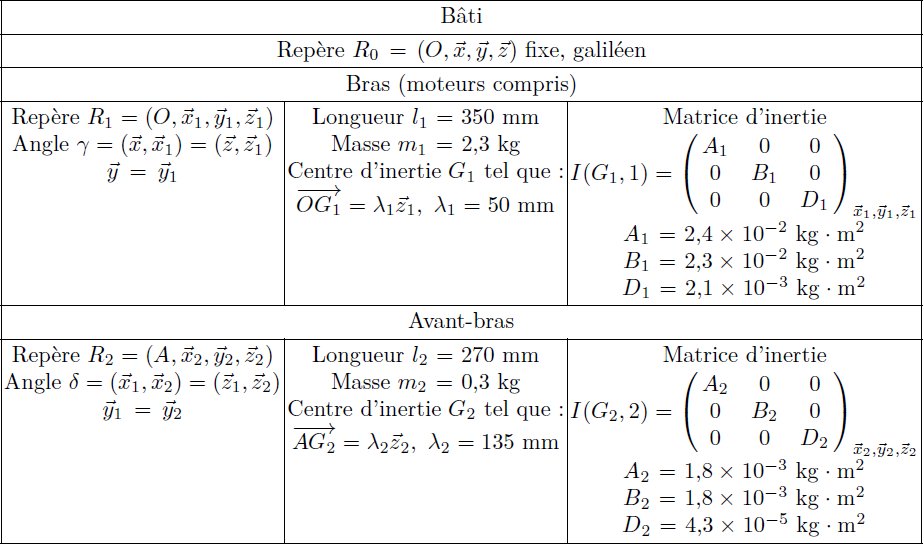
\includegraphics[width=1.0\linewidth]{fig_06}
\end{center}



\subsection*{Modélisation et étude des performances du système avec correction IMC}

\begin{obj}
Améliorer la rapidité tout en atténuant la perturbation sinusoïdale.
\end{obj}

Pour améliorer l’atténuation de la perturbation sinusoïdale, il est possible de changer la
structure de l’asservissement et d’opter pour une correction IMC (Internal Model Corrector)
dont le schéma-blocs est donné sur la figure suivante.

\begin{center}
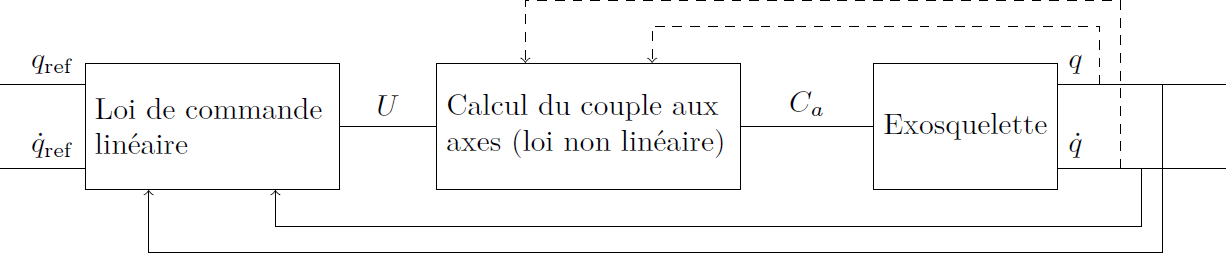
\includegraphics[width=1.0\linewidth]{fig_07}
\end{center}

Avec $F(p)$ la fonction de transfert d’un filtre de la forme $F(p) = \dfrac{1}{\left(1+Tp\right)^2}$ et la fonction de
transfert $H(p) =\dfrac{1}{m_S p^2 + b_S p + k_e}$.



La grandeur de sortie $X_v(p)$ peut s’exprimer par l’équation : $X_v(p) = A(p)X_m(p) + B(p)Q(p)$ avec 
$A(p) = \dfrac{1}{\left(1+Tp\right)^2}$ et $B(p)=\dfrac{Tp\left(2+Tp \right)}{\left(1+Tp\right)^2}$.



\question{Indiquer s’il faut augmenter ou diminuer la valeur de $T$ pour améliorer le temps de réponse
consécutif à un échelon de consigne $x_m(t) = x_0$ (on prendra $Q(p) = 0$ pour cette question).
Justifier votre réponse. En déduire la valeur limite de $T$ permettant de satisfaire l’exigence de
«~rapidité~».}
\ifprof
\begin{corrige}
%On a $Q(p)=0$. On note $\varepsilon_1(p)$ la sortie du premier comparateur et $\varepsilon_2(p)$ la sortie du comparateur de la chaîne de retour.
%
%$X_v(p)=\varepsilon_1(p)\dfrac{1}{H(p)}F(p) H(p)=\varepsilon_1(p)F(p)$,
%
%$\varepsilon_1(p)= X_m(p)-\varepsilon_2(p)$,
%
%$\varepsilon_2(p)= X_v(p)-\varepsilon_1(p)\dfrac{1}{H(p)}F(p) H(p)=X_v(p)-\varepsilon_1(p)F(p)$.
%
%Des deux précédentes équations, il vient $\varepsilon_1(p)= X_m(p)-X_v(p)+\varepsilon_1(p)F(p)$ 
%$\Leftrightarrow \varepsilon_1(p)\left( 1-F(p)\right)=X_m(p)-X_v(p)$ 
%$\Leftrightarrow \varepsilon_1(p) =\dfrac{X_m(p)-X_v(p)}{ 1-F(p)}$.
%
%On a donc 
%$X_v(p)=\dfrac{X_m(p)-X_v(p)}{ 1-F(p)}F(p)$
%
%$\Leftrightarrow X_v(p)\left(1+ \dfrac{F(p)}{ 1-F(p)}\right)=\dfrac{X_m(p)}{ 1-F(p)}$
%$\Leftrightarrow X_v(p)\dfrac{1}{ 1-F(p)}=\dfrac{X_m(p)}{ 1-F(p)}$ et $X_m(p)=X_v(p)$.

En utilisant la formulation proposée, on a $X_v(p) = A(p)X_m(p)  =\dfrac{X_m(p) }{\left(1+Tp\right)^2} $.

Pour améliorer le temps de réponse du système, il faut diminuer $T$. 

\textbf{Justification}
On a $G(p)=\dfrac{1}{1+T^2p^2 +2Tp}$. On a donc $\dfrac{1}{\omega_0^2}=T^2$ et $\dfrac{2\xi}{\omega_0}=2T$. On a donc $\omega_0=\dfrac{1}{T}$ et $\xi = 1$.

Pour $\xi=1$, $t_{5\%}\omega_0 = 5$. Ainsi pour réduire le temps de réponse à 5\% il faut augmenter $\omega_0$ et donc diminuer $T$.

Pour un temps de réponse à 5\% de \SI{0,1}{s}, il faut $\omega_0 = \dfrac{5}{0,1}=\SI{50}{rad.s^{-1}}$ et $T=\SI{0,02}{s}$ (valeur maximale).

\end{corrige}
\else
\fi

\question{Le diagramme de Bode de $B(j\omega)$ pour $T = \SI{1}{s}$ est donné ci-après. Indiquer sur la copie s’il faut augmenter ou diminuer la valeur de $T$ pour minimiser l’effet de
la perturbation sur l’intervalle $[\SI{1,25}{rad.s^{-1}};\SI{12,5}{rad.s^{-1}}]$. Justifier votre réponse. En déduire
la valeur limite de $T$ permettant de satisfaire l’atténuation de la perturbation liée à l’exigence
de « précision » sur cet intervalle.}
\ifprof
\begin{corrige} 
On a  $B(p)=\dfrac{Tp\left(2+Tp \right)}{\left(1+Tp\right)^2}$.

Pour minimiser l'effet de la perturbation, il faut que décaler la cassure vers la droite. D'après le cahier des charges, l'effet de la perturbation doit être divisé par 100. L'atténuation en dB doit donc être de $20\log \dfrac{1}{100} = -\SI{40}{dB}$. 

Il faut donc chercher $T$ pour lequel le gain est de \SI{-40}{dB}. En passant $B(p)$ sous forme canonique et en se plaçant en basse fréquence, on a $B(p)\simeq 2Tp$. On a donc $B_{\text{dB}}(\omega)=20\log \left(2T\omega \right)$. 

On veut $B_{\text{dB}}(12,5)=20\log \left(2T\times 12,5\right) < -40$
soit $\log \left(2T\times 12,5\right) < -2$ $\Rightarrow  2T\times 12,5< e^{-2}$
$\Rightarrow  T< e^{-2}/25$ et $T<\SI{0,005}{s}$. 

%la cassure ait lieu après \SI{12,5}{rad.s^{-1}}. Pour cela il faut diminuer $T$. On peut prendre $T=1/12,5=\SI{0,08}{s}$.
\end{corrige}
\else
\fi

\begin{center}
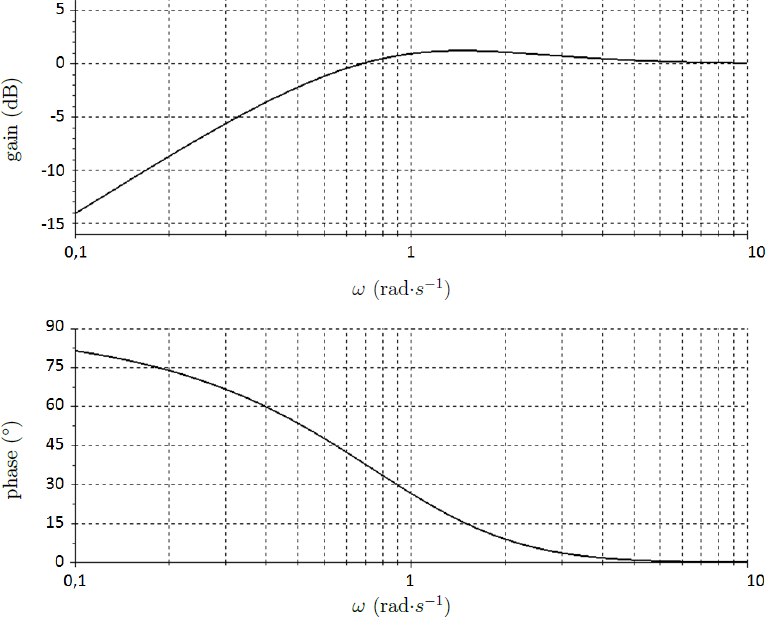
\includegraphics[width=1.0\linewidth]{dr_04}
\end{center}

\ifcolle
\else
\footnotesize
\begin{enumerate}
\item $H(p)=\dfrac{K_aH_s(p)}{1+k_e H_S(p)}$ et $H_t(p)=\dfrac{1}{1+k_e H_s(p)}$.
\item $K=\dfrac{1}{1+k_e}$, $\omega_0=\sqrt{\dfrac{1+k_e}{m_s}}$, $\xi=\dfrac{b_s}{2\sqrt{m_s\left(1+k_e\right)}}$.
\item .
\item .
\item .
\item $K_{i \text{max}} = 133$.
\item $G_{\text{dB max} } = -\SI{30}{dB} $.
\item $T\leq \SI{0,02}{s}$.
\item $T\leq \SI{0,4}{ms}$.
\end{enumerate}
\normalsize
\fi


\end{multicols}

\begin{center}
%\includegraphics[width=1.0\linewidth]{}
\end{center}
%\end{document}
%
%\question{}
%\begin{center}
%\includegraphics[width=\linewidth]{}
%%\textit{}
%\end{center}
%
%